%%%%%%%%%%%%%%%%%%%%%%%%%%%%%%%%%%%%%%%%%%%%%%%%%%%%%%%%%%%%%%%
\chapter{Boundary and Initial Conditions}\label{}
%%%%%%%%%%%%%%%%%%%%%%%%%%%%%%%%%%%%%%%%%%%%%%%%%%%%%%%%%%%%%%%

\section{Boundary Conditions}
%%%%%%%%%%%%%%%%%%%%%%%%%%%%%%%%%%%%%%%%%%%%%%%%%%%%%%%%%%%%%%%

\subsection{Energy balance equation}

\subsubsection{Dirichlet}

\begin{center}
\begin{longtable}{|p {3.0 cm}|p {5.0 cm}|p {1 cm}|p{1 cm}|p{1.1 cm}|p{1.1 cm}|p{1 cm}|}
\hline
\textbf{Keyword} & \textbf{Description} & \textbf{M. U.} & \textbf{range} & \textbf{Default Value} & \textbf{Sca / Vec} & \textbf{Log / Num} \\ \hline
\endfirsthead
\hline
\multicolumn{7}{| c |}{continued from previous page} \\
\hline
\textbf{Keyword} & \textbf{Description} & \textbf{M. U.} & \textbf{range} & \textbf{Default Value} & \textbf{Sca / Vec} & \textbf{Log / Num} \\ \hline
\endhead
\hline
\multicolumn{7}{| c |}{{continued on next page}}\\ 
\hline
\endfoot
\endlastfoot
\hline
ZeroTempAmplitDepth \index{ZeroTempAmplitDepth} & Zero annual amplitude depth (ZAA): depth at which the annual temperature remains constant. It is used as the bottom boundary condition of the heat equation. The Zero flux condition can be assigned setting this parameter at a very high value & mm &  & 1.00E+20 & sca & num \\ \hline
ZeroTempAmplitTemp \index{ZeroTempAmplitTemp} & Temperature at the depth assigned above & $^\circ$C &  & 20 & sca & num \\ \hline
\caption{Keywords of boundary condition for the energy balance equation}
\label{BC1}
\end{longtable}
\end{center}


\subsubsection{Neumann}

\begin{center}
\begin{longtable}{|p {3.8 cm}|p {4.2 cm}|p {1 cm}|p{1 cm}|p{1.1 cm}|p{1.1 cm}|p{1 cm}|}
\hline
\textbf{Keyword} & \textbf{Description} & \textbf{M. U.} & \textbf{range} & \textbf{Default Value} & \textbf{Sca / Vec} & \textbf{Log / Num} \\ \hline
\endfirsthead
\hline
\multicolumn{7}{| c |}{continued from previous page} \\
\hline
\textbf{Keyword} & \textbf{Description} & \textbf{M. U.} & \textbf{range} & \textbf{Default Value} & \textbf{Sca / Vec} & \textbf{Log / Num} \\ \hline
\endhead
\hline
\multicolumn{7}{| c |}{{continued on next page}}\\ 
\hline
\endfoot
\endlastfoot
\hline
BottomBoundaryHeatFlux \index{BottomBoundaryHeatFlux} & Incoming heat flux at the bottom boundary of the soil domain (geothermal heat flux) & W m$^{-2}$ &  & 0 & sca & num \\ \hline
\caption{Keywords of boundary condition for the energy balance equation}
\label{BC2}
\end{longtable}
\end{center}


\subsection{Water balance equation}

\subsubsection{Neumann}
\begin{center}
\begin{longtable}{|p {3.7 cm}|p {4.3 cm}|p {1 cm}|p{1 cm}|p{1.1 cm}|p{1.1 cm}|p{1 cm}|}
\hline
\textbf{Keyword} & \textbf{Description} & \textbf{M. U.} & \textbf{range} & \textbf{Default Value} & \textbf{Sca / Vec} & \textbf{Log / Num} \\ \hline
\endfirsthead
\hline
\multicolumn{7}{| c |}{continued from previous page} \\
\hline
\textbf{Keyword} & \textbf{Description} & \textbf{M. U.} & \textbf{range} & \textbf{Default Value} & \textbf{Sca / Vec} & \textbf{Log / Num} \\ \hline
\endhead
\hline
\multicolumn{7}{| c |}{{continued on next page}}\\ 
\hline
\endfoot
\endlastfoot
\hline
FreeDrainageAtBottom \index{FreeDrainageAtBottom} & Boundary condition on Richards' equation at the bottom border (1: free drainage, 0: no flux) & - & 0,1 & 0 & sca & num \\ \hline
FreeDrainageAtLateralBorder \index{FreeDrainageAtLateralBorder} & Boundary condition on Richards' equation at the lateral border (1: free drainage, 0: no flux) & - & 0,1 & 1 & sca & num \\ \hline
PointDepthFreeSurface \index{PointDepthFreeSurface} & depth of the trench that simulates the drainage of a soil column through a weir. The deeper the trench, the higher the drainage. Valid in 1D simulations & mm &  & NA & vec & num \\ \hline
\caption{Keywords of boundary condition for the energy balance equation}
\label{BC3}
\end{longtable}
\end{center}






%%%%%%%%%%%%%%%%%%%%%%%%%%%%%%%%%%%%%%%%%%%%%%%%%%%%%%%%%%%%%%%
\section{Initial Conditions}
%%%%%%%%%%%%%%%%%%%%%%%%%%%%%%%%%%%%%%%%%%%%%%%%%%%%%%%%%%%%%%%

\subsection{Snow}

\begin{center}
\begin{longtable}{|p {3.0 cm}|p {4.5 cm}|p {1 cm}|p{1 cm}|p{1.1 cm}|p{1.1 cm}|p{1 cm}|}
\hline
\textbf{Keyword} & \textbf{Description} & \textbf{M. U.} & \textbf{range} & \textbf{Default Value} & \textbf{Scalar / Vector} & \textbf{Log / Num} \\ \hline
\endfirsthead
\hline
\multicolumn{7}{| c |}{continued from previous page} \\
\hline
\textbf{Keyword} & \textbf{Description} & \textbf{M. U.} & \textbf{range} & \textbf{Default Value} & \textbf{Scalar / Vector} & \textbf{Log / Num} \\ \hline
\endhead
\hline
\multicolumn{7}{| c |}{{continued on next page}}\\ 
\hline
\endfoot
\endlastfoot
\hline
InitSWE \index{InitSWE} & Initial snow water equivalent (SWE) - used if no snow map is given & kg m$^{-2}$ &  & 0 & sca & num \\ \hline
InitSnowDensity \index{InitSnowDensity} & Initial snow density - uniform with depth & kg m$^{-3}$ &  & 200 & sca & num \\ \hline
InitSnowTemp \index{InitSnowTemp} & Initial snow temperature - uniform with depth & $^\circ$C &  & -3 & sca & num \\ \hline
InitSnowAge \index{InitSnowAge} & Initial snow age & days &  & 0 & sca & num \\ \hline
\caption{Keywords for the input of initial conditions}
\label{IC1}
\end{longtable}
\end{center}

\subsection{Glacier}

\begin{center}
\begin{longtable}{|p {3.0 cm}|p {4.5 cm}|p {1 cm}|p{1 cm}|p{1.1 cm}|p{1.1 cm}|p{1 cm}|}
\hline
\textbf{Keyword} & \textbf{Description} & \textbf{M. U.} & \textbf{range} & \textbf{Default Value} & \textbf{Scalar / Vector} & \textbf{Log / Num} \\ \hline
\endfirsthead
\hline
\multicolumn{7}{| c |}{continued from previous page} \\
\hline
\textbf{Keyword} & \textbf{Description} & \textbf{M. U.} & \textbf{range} & \textbf{Default Value} & \textbf{Scalar / Vector} & \textbf{Log / Num} \\ \hline
\endhead
\hline
\multicolumn{7}{| c |}{{continued on next page}}\\ 
\hline
\endfoot
\endlastfoot
\hline
InitGlacierDepth \index{InitGlacierDepth} & Initial glacier depth - used if no snow map is given & mm &  & 0 & sca & num \\ \hline
InitGlacierDensity \index{InitGlacierDensity} & Initial glacier density - uniform with depth & kg m$^{-3}$ &  & 800 & sca & num \\ \hline
InitGlacierTemp \index{InitGlacierTemp} & Initial glacier temperature - uniform with depth & $^\circ$C &  & -3 & sca & num \\ \hline
\caption{Keywords for the input of initial conditions}
\label{IC2}
\end{longtable}
\end{center}


\subsection{Soil / Rock}

\subsubsection{Water balance equation}
\begin{center}
\begin{longtable}{|p {4.9 cm}|p {2.6 cm}|p {1 cm}|p{1 cm}|p{1.1 cm}|p{1.1 cm}|p{1 cm}|}
\hline
\textbf{Keyword} & \textbf{Description} & \textbf{M. U.} & \textbf{range} & \textbf{Default Value} & \textbf{Scalar / Vector} & \textbf{Log / Num} \\ \hline
\endfirsthead
\hline
\multicolumn{7}{| c |}{continued from previous page} \\
\hline
\textbf{Keyword} & \textbf{Description} & \textbf{M. U.} & \textbf{range} & \textbf{Default Value} & \textbf{Scalar / Vector} & \textbf{Log / Num} \\ \hline
\endhead
\hline
\multicolumn{7}{| c |}{{continued on next page}}\\ 
\hline
\endfoot
\endlastfoot
\hline
InitWaterTableHeightOverTopoSurface \index{InitWaterTableHeightOverTopoSurface} & initial condition on water table depth (positive downwards from ground surface). Used if InitSoilPressure is void & mm &  & 0 & sca & num \\ \hline
InitSoilPressure \index{InitSoilPressure} &  & mm &  & NA & vec & num \\ \hline
InitSoilPressureBedrock \index{InitSoilPressureBedrock} &  & mm &  & NA & vec & num \\ \hline
\caption{Keywords for the input of initial conditions}
\label{IC3}
\end{longtable}
\end{center}

\subsubsection{Energy balance equation}
\begin{center}
\begin{longtable}{|p {3.0 cm}|p {4.5 cm}|p {1 cm}|p{1 cm}|p{1.1 cm}|p{1.1 cm}|p{1 cm}|}
\hline
\textbf{Keyword} & \textbf{Description} & \textbf{M. U.} & \textbf{range} & \textbf{Default Value} & \textbf{Scalar / Vector} & \textbf{Log / Num} \\ \hline
\endfirsthead
\hline
\multicolumn{7}{| c |}{continued from previous page} \\
\hline
\textbf{Keyword} & \textbf{Description} & \textbf{M. U.} & \textbf{range} & \textbf{Default Value} & \textbf{Scalar / Vector} & \textbf{Log / Num} \\ \hline
\endhead
\hline
\multicolumn{7}{| c |}{{continued on next page}}\\ 
\hline
\endfoot
\endlastfoot
\hline
IInitSoilTemp \index{IInitSoilTemp} &  & $^\circ$C &  & 5 & vec & num \\ \hline
InitSoilTempBedrock \index{InitSoilTempBedrock} &  & $^\circ$C &  & 5 & vec & num \\ \hline
\caption{Keywords for the input of initial conditions settable in geotop.inpts}
\label{IC4}
\end{longtable}
\end{center}


%\begin{figure}[h!]
%\begin{center}
%  \begin{minipage}[c]{.3\textwidth}
%    \centering
%    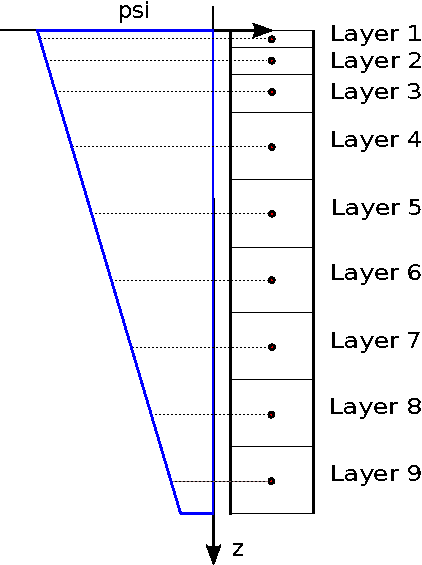
\includegraphics[width=1\textwidth]{./images/pic_ICBC/suolo_pai.pdf}
%  \end{minipage}%
%\end{center}
%\textsl{\caption{Soil/rock initial condition on suction head $\psi$}\label{soiil}}
%\end{figure}

%\begin{figure}[h,t,b]
%\begin{center}
%  \begin{minipage}[c]{.4\textwidth}
%    \centering
%    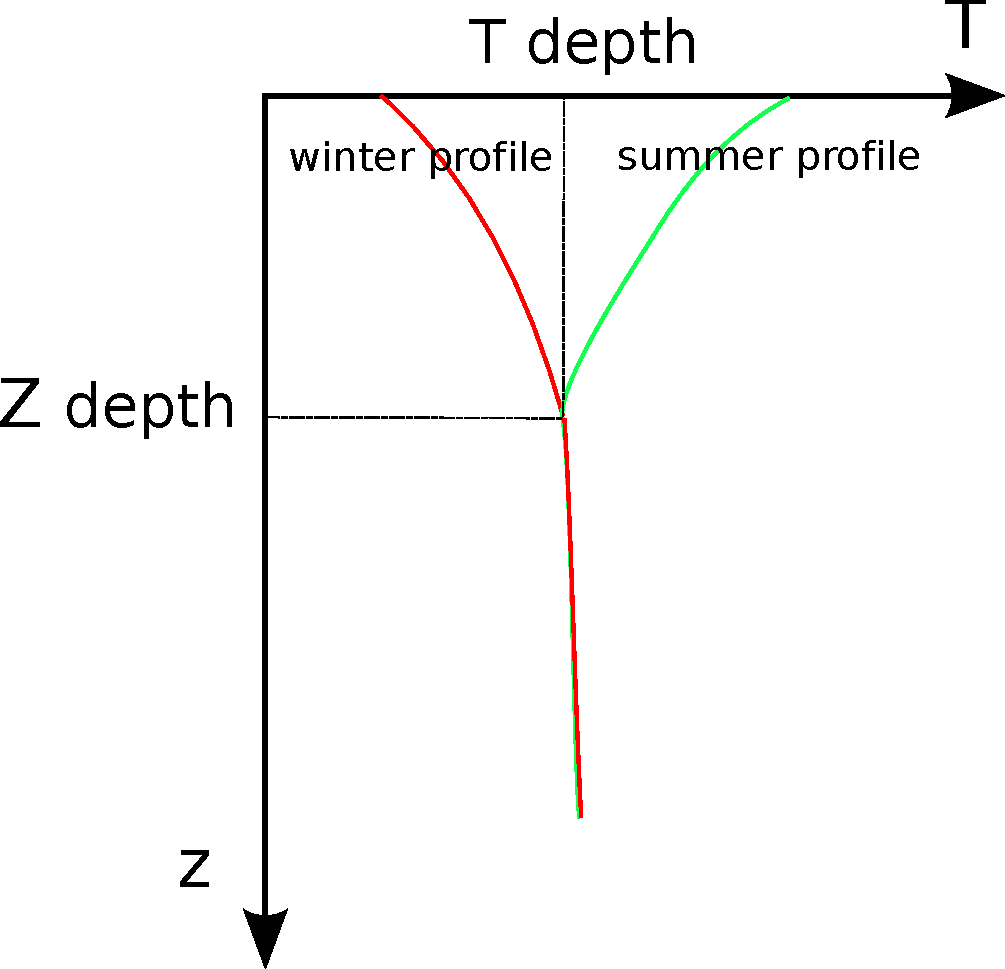
\includegraphics[width=1\textwidth]{./images/pic_ICBC/temperature.pdf}
%  \end{minipage}%
%\end{center}
%\textsl{\caption{Zero annual amplitude depth}\label{}}
%\end{figure}

